%%%%%%%%%%%%%%%%%%%%%%%%%%%%%%%%%%%%%%%%%%%%%%%%
% Grenzwerte von Funktionen, Stetigkeit        
%%%%%%%%%%%%%%%%%%%%%%%%%%%%%%%%%%%%%%%%%%%%%%%%
\section{Grenzwerte von Funktionen\formelbuchorange{53}}

	\subsection{Berechnung von Grenzwerten\formelbuchorange{56}}
		Technik des $Erweiterns$: $\lim\limits_{n\to\infty} \frac{n}{n^2}$
		$\Longrightarrow $ Erweitern mit
		$\frac{1}{n^2} \Longrightarrow \lim\limits_{n\to\infty}$
		$\frac{\frac{n}{n^2}}{\frac{n^2}{n^2}} =$
		$\lim\limits_{n\to\infty} \frac{1}{n} = 0 $\\\\
		$Binomische Formel$: $\quad\lim\limits_{n\to\infty}\sqrt{n+1}-\sqrt{n} =$ 
		$\lim\limits_{n\to\infty} $
		$\frac{(\sqrt{n+1}-\sqrt{n})(\sqrt{n+1}+\sqrt{n})}{\sqrt{n+1}+\sqrt{n}} = $
		$\lim\limits_{n\to\infty} \frac{n+1-n}{\sqrt{n+1}+\sqrt{n}}= 0$

	\subsubsection{Spezielle Grenzwert S"atze}
		\begin{minipage}[t]{6 cm}
			$\lim\limits_{x\to x_0} |f(x)| = |\lim\limits_{x\to x_0} f(x)| = |g|$\\
		\end{minipage}
		\begin{minipage}[t]{6 cm}
			$\lim\limits_{x\to x_0} (f(x))^n = (\lim\limits_{x\to x_0} f(x))^n = g^n$ \\
		\end{minipage}
		\begin{minipage}[t]{6 cm}
			$\lim\limits_{x\to x_0} \sqrt[n]{f(x)} = \sqrt[n]{\lim\limits_{x\to x_0} f(x)} = \sqrt[n]{g}$
		\end{minipage}

	\subsubsection{Einschliessungsprinzip\formelbuchorange{55}}
		\begin{minipage}[t]{9 cm}
			$\lim\limits_{n \to \infty} a_n = \lim\limits_{n \to \infty} b_n = g \wedge a_n, b_n$ sind konvergent\\
		\end{minipage}
		\begin{minipage}[t]{9 cm}
			$a_n \leq c_n \leq b_n \Rightarrow \lim\limits_{n \to \infty} c_n = g$
		\end{minipage}

	\begin{figure}[ht]
		\begin{minipage}[b]{10.4 cm}
			\subsection{Links-/Rechtsseitiger Grenzwert\formelbuchorange{54}}
				Rechtsseitiger Grenzwert: $\lim\limits_{x \to x_0^+} f(x) = \lim\limits_{x \downarrow x_0}$
				$f(x) = g^+$\\
				Linksseitiger Grenzwert: $\lim\limits_{x \to x_0^-} f(x) = \lim\limits_{x \uparrow x_0}$
				$f(x) = g^-$

			\subsection{Konvergenz, Divergenz\formelbuchorange{474}}
				Konvergenz: $g^+ = g^- = g \in \mathbb{R}$ oder: monoton und beschr"ankt\\
				Bestimmte Divergenz: $g = +\infty$ oder: $g = -\infty$\\ 
				Unbestimmte Divergenz: Es existiert kein Grenzwert\\
				\small{($g$ f"ur Grenzwert)}

			\subsection{Stetigkeit\formelbuchorange{59}}
				"`Wenn man die Funktion mit einem Strich zeichnen kann"':\\
				$\lim\limits_{x \to x_0} f(x) = f(x_0)$
  		\end{minipage}
  		\begin{minipage}[b]{8 cm}
    		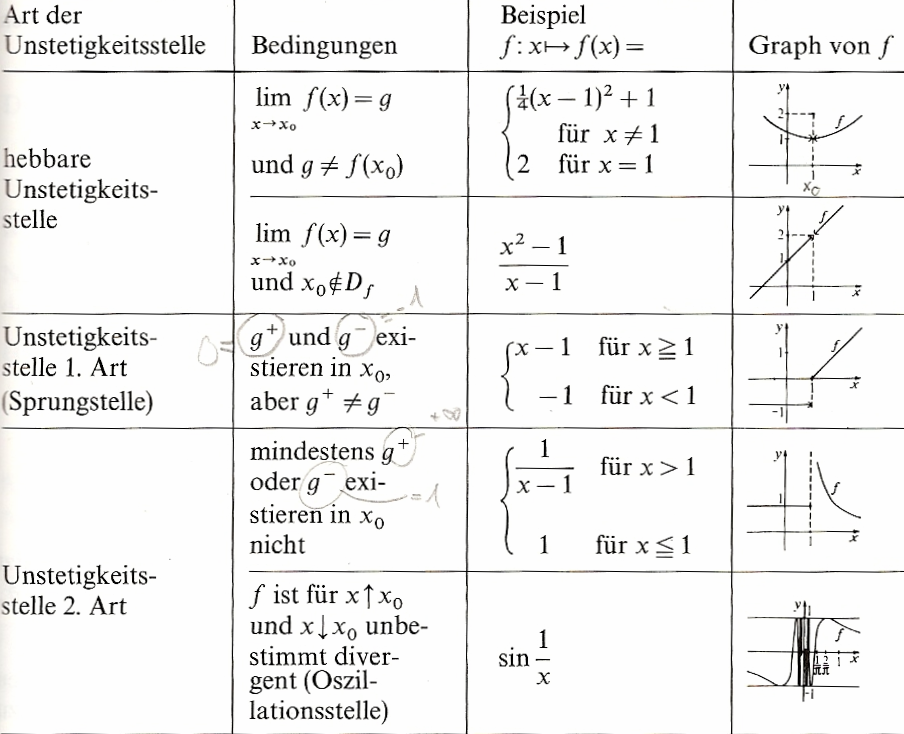
\includegraphics[width=8 cm]{./bilder/grenzwerte_unstetigkeitsstellen.png}
  		\end{minipage}
	\end{figure}
	
	\subsection{"Ubertragungsprinzip}
				\begin{tabbing}
		--------\=---------------------------------------------------\=---------------------------------------------------\=---------------------------------------------------\=\kill
			$f$ besitzt genau an der Stelle $x_0$ den Grenzwert $g$, wenn f"ur jede gegen $x_0$ konvergente Folge $<x_n>$ gilt: $\lim\limits_{n\to\infty}f(x_n)=g$\\
			Bsp: \>
			$f(x)=x-[x]$ und $x_0=-1$\>
			$x_n=-1-\frac{1}{n} \rightarrow \lim\limits_{n\to\infty}(x_n)=-1$\>
			$x_n'=-1+\frac{1}{n} \rightarrow \lim\limits_{n\to\infty}(x_n')=-1$\\	
			\>wenn nun gilt\\
			\>$\lim\limits_{n\to\infty}f(x_n)=\lim\limits_{n\to\infty}(-1-\frac{1}{n}-[-1-\frac{1}{n}])=1\neq\lim\limits_{n\to\infty}f(x_n')=\lim\limits_{n\to\infty}(-1+\frac{1}{n}-[-1+\frac{1}{n}])=0$\\
			\>Dann besitzt die Funktion $f(x)$ an der Stelle $x_0$ keinen Grenzwert $g$.
		\end{tabbing}

	\subsection{Spezielle Grenzwerte\formelbuchorange{58}}
  		\begin{minipage}[c]{6.33cm}
			$\lim\limits_{x \to 0} \frac{\sin{x}}{x} = 1 $
  		\end{minipage}
  		\begin{minipage}[c]{6.33cm}
			$ \lim\limits_{x \to \infty} \frac{x^{\alpha}}{a^{\beta x}} = 0 \:(a>1;\:\alpha, \beta > 0 ) $
  		\end{minipage}
  		\begin{minipage}[c]{6.33cm}
			$ \lim\limits_{x \to \infty} \frac{x^\alpha}{a^{\beta x}} = 0 $
  		\end{minipage} \\ \\
  		\begin{minipage}[c]{6.33cm}
			$ \lim\limits_{x \to \infty} (1+\frac{a}{x})^x=e^a $
  		\end{minipage}
  		\begin{minipage}[c]{6.33cm}
			$ \lim\limits_{x \to 0} (1+x)^{\frac{1}{x}}=e $
  		\end{minipage}
  		\begin{minipage}[c]{6.33cm}
				$ \lim\limits_{x \to 0} \frac{a^x-1}{x}=\ln a $
  		\end{minipage} \\ \\
  		\begin{minipage}[c]{6.33cm}
				$ \lim\limits_{x \to 0} \frac{\log_a(x+1)}{x} = \frac{1}{\ln a} $
  		\end{minipage}
  		\begin{minipage}[c]{6.33cm}
			$ \lim\limits_{x \to \infty} \frac{(\ln x)^\alpha}{x^{\beta}} = 0 $
  		\end{minipage}
  		\begin{minipage}[c]{6.33cm}
			$ \lim\limits_{x \to 2} \ln{\sqrt{\frac{x^2-4}{x-2}}} = \ln{2} $
  		\end{minipage} \\ \\
  		\begin{minipage}[c]{6.33cm}
			$ \lim\limits_{x \to 1} \frac{\ln{x}}{x-1} = 1 $
  		\end{minipage}
  		\begin{minipage}[c]{6.33cm}
			$ \lim\limits_{x \to 0+} x \ln{x} = 0 $
  		\end{minipage}
  		\begin{minipage}[c]{6.33cm}
			$ \lim\limits_{x \to 0} \frac{e^x-1}{x}=1 $
  		\end{minipage} \\ \\
  		\begin{minipage}[c]{6.33cm}
			$ \lim\limits_{x \to 0} \frac{x}{1-e^{-x}}=1 $
  		\end{minipage}
  		\begin{minipage}[c]{6.33cm}
			$ \lim\limits_{x \to \infty} \sum_{k=0}^n q^k = \begin{cases}+\infty &q \geq 1\\ \frac{1}{1-q} &|q|<1\end{cases} $
  		\end{minipage}
  		\begin{minipage}[c]{6.33cm}
			$ \lim\limits_{\alpha \to 0} \frac{(1+x)^{\alpha}-1}{x} = \alpha $
  		\end{minipage} \\ \\
  		\begin{minipage}[c]{6.33cm}
			$ \lim\limits_{x \to \infty} \frac{x^n}{n!} = 0 \:(x>0) $
  		\end{minipage}
  		\begin{minipage}[c]{6.33cm}
			$ \lim\limits_{x \to \infty} \frac{x^k}{q^x}=0 \:(q>1; \:k\in \mathbb{N}) $
  		\end{minipage}
  		\begin{minipage}[c]{6.33cm}
			$ \lim\limits_{x \to \infty} \sqrt[x]{p}=1 $
  		\end{minipage} \\ \\
  		\begin{minipage}[c]{6.33cm}
			$ \lim\limits_{x \to \infty} \sqrt[x]{x}=1 $
  		\end{minipage}

	\subsection{Asymptotenbestimmung\formelbuchorange{15}}
		Ausrechnen der Asymptote einer gebrochen rationalen Funktion $r: x \mapsto r(x)=\frac{P_m(x)}{Q_n(x)}$:
		\begin{tabbing}
		-----------------------------------\=-----------------------------------\=-----------------------------------\=\kill
			\>$m < n$ \>$m=n$ \>$m > n$\\
			$\lim\limits_{x\to \pm \infty} r(x) = $ 
			\>0 \>$\frac{a_m}{b_n}$ \> $+\infty$ oder $-\infty$\\
			Asymptote 
			\>x-Achse \>Parallel zur x-Achse \>Ganzrationaler Teil\\
			\> \>$y = g(x) = \frac{a_m}{b_n}$ \>der Polynomdivision\formelbuchorange{15}
		\end{tabbing}